\begin{figure}[!ht]
    \centering

\tikzset{every picture/.style={line width=0.75pt}} %set default line width to 0.75pt        

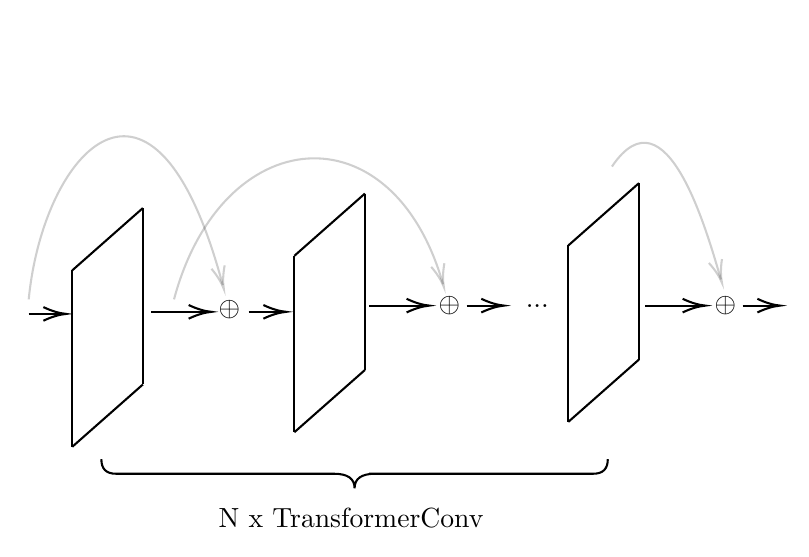
\begin{tikzpicture}[x=0.75pt,y=0.75pt,yscale=-1,xscale=1]
%uncomment if require: \path (0,300); %set diagram left start at 0, and has height of 300

%Straight Lines [id:da8903776144061866] 
\draw    (73,93) -- (107,63) ;
%Straight Lines [id:da2760973702056343] 
\draw    (73,178) -- (107,148) ;
%Straight Lines [id:da36156173030181205] 
\draw    (73,93) -- (73,178) ;
%Straight Lines [id:da31935074154742293] 
\draw    (107,63) -- (107,148) ;
%Curve Lines [id:da5901112440809217] 
\draw [color={rgb, 255:red, 0; green, 0; blue, 0 }  ,draw opacity=0.19 ]   (52,107) .. controls (58.97,35.36) and (112.46,-23.41) .. (145.5,100.12) ;
\draw [shift={(146,102)}, rotate = 255.32] [color={rgb, 255:red, 0; green, 0; blue, 0 }  ,draw opacity=0.19 ][line width=0.75]    (10.93,-3.29) .. controls (6.95,-1.4) and (3.31,-0.3) .. (0,0) .. controls (3.31,0.3) and (6.95,1.4) .. (10.93,3.29)   ;
%Straight Lines [id:da5316335291603521] 
\draw    (111,113) -- (138,113) ;
\draw [shift={(140,113)}, rotate = 180] [color={rgb, 255:red, 0; green, 0; blue, 0 }  ][line width=0.75]    (10.93,-3.29) .. controls (6.95,-1.4) and (3.31,-0.3) .. (0,0) .. controls (3.31,0.3) and (6.95,1.4) .. (10.93,3.29)   ;
%Straight Lines [id:da9890926899340573] 
\draw    (158,113) -- (174,113) ;
\draw [shift={(176,113)}, rotate = 180] [color={rgb, 255:red, 0; green, 0; blue, 0 }  ][line width=0.75]    (10.93,-3.29) .. controls (6.95,-1.4) and (3.31,-0.3) .. (0,0) .. controls (3.31,0.3) and (6.95,1.4) .. (10.93,3.29)   ;
%Straight Lines [id:da39728945983861974] 
\draw    (180,86) -- (214,56) ;
%Straight Lines [id:da546357430615998] 
\draw    (180,171) -- (214,141) ;
%Straight Lines [id:da738375355055665] 
\draw    (180,86) -- (180,171) ;
%Straight Lines [id:da3679147122770259] 
\draw    (214,56) -- (214,141) ;
%Straight Lines [id:da5699108183848012] 
\draw    (52,114) -- (68,114) ;
\draw [shift={(70,114)}, rotate = 180] [color={rgb, 255:red, 0; green, 0; blue, 0 }  ][line width=0.75]    (10.93,-3.29) .. controls (6.95,-1.4) and (3.31,-0.3) .. (0,0) .. controls (3.31,0.3) and (6.95,1.4) .. (10.93,3.29)   ;
%Straight Lines [id:da43476534361548547] 
\draw    (216,110) -- (243,110) ;
\draw [shift={(245,110)}, rotate = 180] [color={rgb, 255:red, 0; green, 0; blue, 0 }  ][line width=0.75]    (10.93,-3.29) .. controls (6.95,-1.4) and (3.31,-0.3) .. (0,0) .. controls (3.31,0.3) and (6.95,1.4) .. (10.93,3.29)   ;
%Straight Lines [id:da04916512065436518] 
\draw    (263,110) -- (279,110) ;
\draw [shift={(281,110)}, rotate = 180] [color={rgb, 255:red, 0; green, 0; blue, 0 }  ][line width=0.75]    (10.93,-3.29) .. controls (6.95,-1.4) and (3.31,-0.3) .. (0,0) .. controls (3.31,0.3) and (6.95,1.4) .. (10.93,3.29)   ;
%Straight Lines [id:da7000406032171446] 
\draw    (312,81) -- (346,51) ;
%Straight Lines [id:da08237114236162735] 
\draw    (312,166) -- (346,136) ;
%Straight Lines [id:da4267402686351852] 
\draw    (312,81) -- (312,166) ;
%Straight Lines [id:da24889074507156195] 
\draw    (346,51) -- (346,136) ;
%Straight Lines [id:da11047393229022784] 
\draw    (349,110) -- (376,110) ;
\draw [shift={(378,110)}, rotate = 180] [color={rgb, 255:red, 0; green, 0; blue, 0 }  ][line width=0.75]    (10.93,-3.29) .. controls (6.95,-1.4) and (3.31,-0.3) .. (0,0) .. controls (3.31,0.3) and (6.95,1.4) .. (10.93,3.29)   ;
%Straight Lines [id:da8573297385314265] 
\draw    (396,110) -- (412,110) ;
\draw [shift={(414,110)}, rotate = 180] [color={rgb, 255:red, 0; green, 0; blue, 0 }  ][line width=0.75]    (10.93,-3.29) .. controls (6.95,-1.4) and (3.31,-0.3) .. (0,0) .. controls (3.31,0.3) and (6.95,1.4) .. (10.93,3.29)   ;
%Shape: Brace [id:dp7869180953072277] 
\draw   (87,184) .. controls (87,188.67) and (89.33,191) .. (94,191) -- (199,191) .. controls (205.67,191) and (209,193.33) .. (209,198) .. controls (209,193.33) and (212.33,191) .. (219,191)(216,191) -- (324,191) .. controls (328.67,191) and (331,188.67) .. (331,184) ;
%Curve Lines [id:da788508586152133] 
\draw [color={rgb, 255:red, 0; green, 0; blue, 0 }  ,draw opacity=0.19 ]   (333,43) .. controls (359.33,4) and (379,75.27) .. (385.52,97.4) ;
\draw [shift={(386,99)}, rotate = 253.3] [color={rgb, 255:red, 0; green, 0; blue, 0 }  ,draw opacity=0.19 ][line width=0.75]    (10.93,-3.29) .. controls (6.95,-1.4) and (3.31,-0.3) .. (0,0) .. controls (3.31,0.3) and (6.95,1.4) .. (10.93,3.29)   ;
%Curve Lines [id:da5871200774240419] 
\draw [color={rgb, 255:red, 0; green, 0; blue, 0 }  ,draw opacity=0.19 ]   (122,107) .. controls (144.89,21.43) and (227.17,14.07) .. (251.64,99.7) ;
\draw [shift={(252,101)}, rotate = 254.58] [color={rgb, 255:red, 0; green, 0; blue, 0 }  ,draw opacity=0.19 ][line width=0.75]    (10.93,-3.29) .. controls (6.95,-1.4) and (3.31,-0.3) .. (0,0) .. controls (3.31,0.3) and (6.95,1.4) .. (10.93,3.29)   ;

% Text Node
\draw (142,106) node [anchor=north west][inner sep=0.75pt]    {$\oplus $};
% Text Node
\draw (248,104) node [anchor=north west][inner sep=0.75pt]    {$\oplus $};
% Text Node
\draw (290,108) node [anchor=north west][inner sep=0.75pt]   [align=left] {...};
% Text Node
\draw (381,104) node [anchor=north west][inner sep=0.75pt]    {$\oplus $};
% Text Node
\draw (142,206) node [anchor=north west][inner sep=0.75pt]   [align=left] {N x TransformerConv};


\end{tikzpicture}
    \caption{Graph layers overview}
    \label{fig:gnn}
\end{figure}